% Section content template for individual Educative lessons
% This file contains the actual content for a specific section
% Generated from Educative API section content

% Section: Design of a Blob Store
% Section ID: 4910790825476096
% Section Slug: design-of-a-blob-store
% Generated: 2025-12-07T21:37:01.005116

\subsection{High-level design}\label{8T_83u7LMTmjDypviQlsy}
\\
Let\textquotesingle s identify and connect the components of a blob store system. At a high level, the components are clients, front-end servers, and storage disks.

\begin{figure}[htbp]
 \centering
 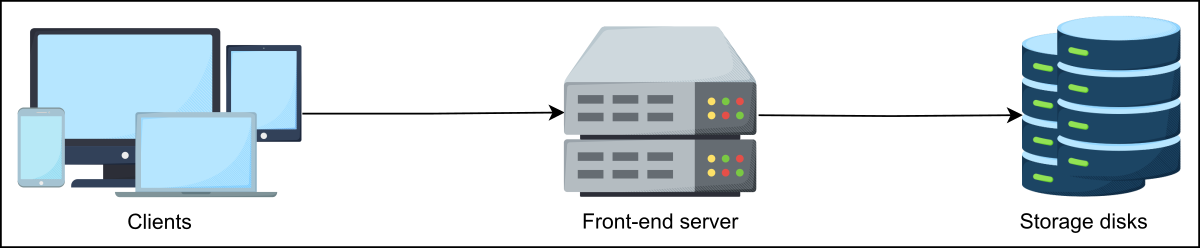
\includegraphics[width=0.5\textwidth]{Images/chapter_20/section_4910790825476096/6431592598077440.png}
 \caption{The high-level design of a blob store}
\end{figure}

The client's requests are received at the front-end servers that process the request. The front-end servers store the client's blob onto the storage disks attached to them.

\subsection{API design}\label{YiVcGUT7bqlv9-KWUFgaW}
\\
Let's look into the API design of the blob store. All of the functions below can only be performed by a registered and authenticated user. For the sake of brevity, we don't include functionalities like registration and authentication of users.

\subsubsection{Create container}\label{DbPvdAQ-ImkxgLt07UaBU}
\\
The \texttt{createContainer} operation creates a new container under~the logged-in account from which this request is being generated.

\begin{lstlisting}[language=JavaScript]
createContainer(containerName)
\end{lstlisting}

\begin{table}[htbp]
\centering
\small
\adjustbox{max width=\textwidth}{
\begin{tabular}{|p{0.171\textwidth}|p{0.779\textwidth}|}
\hline
\textbf{Parameter} & \textbf{Description} \\
\hline
\hline
\texttt{containerName} & This is the name of the container. It should be unique within a storage account. \\
\hline
\end{tabular}
}
\end{table}

\subsubsection{Upload blobs}\label{7KHuCVFgOV06cbEkqz4vk}
\\
The client's data is stored in the form of Bytes in the blob store. The data can be put into a container with the following code:

\begin{lstlisting}[language=JavaScript]
putBlob(containerPath, blobName, data)
\end{lstlisting}

\begin{table}[htbp]
\centering
\small
\adjustbox{max width=\textwidth}{
\begin{tabular}{|p{0.171\textwidth}|p{0.779\textwidth}|}
\hline
\textbf{Parameter} & \textbf{Description} \\
\hline
\hline
\texttt{containerPath} & This is the path of the container in which we upload the blob. It consists of the \texttt{accountID} and \texttt{containerID}. \\
\hline
\texttt{blobName} & This is the name of the blob. It should be unique within a container, otherwise our system will give the blob that was uploaded later a version number. \\
\hline
\texttt{data} & This is a file that the user wants to upload to the blob store. \\
\hline
\end{tabular}
}
\end{table}

\begin{quote}
\textbf{Note:} This API is just a logical way to spell out needs. We might use a multistep streaming call for actual implementation if the data size is very large.
\end{quote}
\subsubsection{Download blobs}\label{0zK4cjqRJXuF9HMvL2Ch4}
\\
Blobs are identified by their unique name or ID.

\begin{lstlisting}[language=JavaScript]
getBlob(blobPath)
\end{lstlisting}

\begin{table}[htbp]
\centering
\small
\adjustbox{max width=\textwidth}{
\begin{tabular}{|p{0.171\textwidth}|p{0.779\textwidth}|}
\hline
\textbf{Parameter} & \textbf{Description} \\
\hline
\hline
\texttt{blobPath} & This is the fully qualified path of the data or file, including its unique ID. \\
\hline
\end{tabular}
}
\end{table}

\subsubsection{Delete blob}\label{6Dm8r3h1fAcmQNM_GKJDP}
\\
The \texttt{deleteBlob} operation marks the specified blob for deletion. The actual blob is deleted during garbage collection.

\begin{lstlisting}[language=JavaScript]
deleteBlob(blobPath)
\end{lstlisting}

\begin{table}[htbp]
\centering
\small
\adjustbox{max width=\textwidth}{
\begin{tabular}{|p{0.171\textwidth}|p{0.779\textwidth}|}
\hline
\textbf{Parameter} & \textbf{Description} \\
\hline
\hline
\texttt{blobPath} & This is the path of the blob that the user wants to delete. \\
\hline
\end{tabular}
}
\end{table}

\subsubsection{List blobs}\label{y9OR2-iae4eYUERptOvMp}
\\
The \texttt{listBlobs} operation returns a list of blobs under the specified container or path.

\begin{lstlisting}[language=JavaScript]
listBlobs(containerPath)
\end{lstlisting}

\begin{table}[htbp]
\centering
\small
\adjustbox{max width=\textwidth}{
\begin{tabular}{|p{0.171\textwidth}|p{0.779\textwidth}|}
\hline
\textbf{Parameter} & \textbf{Description} \\
\hline
\hline
\texttt{containerPath} & This is the path to the container from which the user wants to get the list of blobs. \\
\hline
\end{tabular}
}
\end{table}

\subsubsection{Delete container}\label{tleRe6eXYSMUnHZyvnStq}
\\
The \texttt{deleteContainer} operation marks the specified container for deletion. The container and any blobs in it are deleted later during garbage collection.

\begin{lstlisting}[language=JavaScript]
deleteContainer(containerPath)
\end{lstlisting}

\begin{table}[htbp]
\centering
\small
\adjustbox{max width=\textwidth}{
\begin{tabular}{|p{0.171\textwidth}|p{0.779\textwidth}|}
\hline
\textbf{Parameter} & \textbf{Description} \\
\hline
\hline
\texttt{containerPath} & This is the path to the container that the user wants to delete. \\
\hline
\end{tabular}
}
\end{table}

\subsubsection{List containers}\label{7yLrwdOLKV35Yr9aN0L6S}
\\
The \texttt{listContainers} operation returns a list of the containers under the specified user's blob store account.

\begin{lstlisting}[language=JavaScript]
listContainers(accountID)
\end{lstlisting}

\begin{table}[htbp]
\centering
\small
\adjustbox{max width=\textwidth}{
\begin{tabular}{|p{0.171\textwidth}|p{0.779\textwidth}|}
\hline
\textbf{Parameter} & \textbf{Description} \\
\hline
\hline
\texttt{accountID} & This is the ID of the user who wants to list their containers. \\
\hline
\end{tabular}
}
\end{table}

\begin{quote}
\textbf{Note:} The APIs used to retrieve blobs provide metadata containing size, version number, access privileges, name, and so on.
\end{quote}
\subsection{Detailed design}\label{ljXYJrkelDWSWnKGfAMLh}
\\
We start this section by identifying the key components that we need to complete our blob store design. Then , we look at how these components connect to fulfill our functional requirements.

\subsubsection{Components}\label{g09cVGuIIDaJNBUS6YSAK}
\\
Here is a list of components that we use in the blob store design:

\begin{itemize}
\item
\protect\phantomsection\label{r0axmnG0KhsirIh0As36g}
\textbf{Client:} This is a user or program that performs any of the API functions that are specified.
\item
\protect\phantomsection\label{S_iXIPvNNv_2BxZ3AEbzh}
\textbf{Rate limiter:} A rate limiter limits the number of requests based on the user's subscription or limits the number of requests from the same IP address at the same time. It doesn't allow users to exceed the predefined limit.
\item
\protect\phantomsection\label{zK2MHzZ6erXUA4DdB2K1C}
\textbf{Load balancer:} A load balancer distributes incoming network traffic among a group of servers. It's also used to reroute requests to different regions depending on the location of the user, different data centers within the same region, or different servers within the same data center. \textbf{DNS} load balancing can be used to reroute the requests among different regions based on the location of the user.
\item
\protect\phantomsection\label{h8c8k4TrWCPMUjJut55j4}
\textbf{Front-end servers:} Front-end servers forward the users' requests for adding or deleting data to the appropriate storage servers.
\item
\protect\phantomsection\label{YKbSzlx16jW7XnG1Zr6QL}
\textbf{Data nodes:} Data nodes hold the actual blob data. It's also possible that they contain a part of the blob's data. Blobs are split into small, fixed-size pieces called \textbf{chunks}. A data node can accommodate all of the chunks of a blob or at least some of them.
\item
\protect\phantomsection\label{7S3-Da-4h-U4Tc8bxCJWC}
\textbf{Manager node:} A manager node is the core component that manages all data nodes. It stores information about storage paths and the access privileges of blobs. There are two types of access privileges: private and public. A \emph{private} access privilege means that the blob is only accessible by the account containing that blob. A \emph{public} access privilege means that anyone can access that blob.
\item
\protect\phantomsection\label{-2Wv9ehSf8Od1phyhLn9M}
\textbf{Metadata storage:} Metadata storage is a distributed database that's used by the manager node to store all the metadata. Metadata consists of account metadata, container metadata, and blob metadata.

\begin{itemize}
\item
\emph{\textbf{Account metadata}} contains the account information for each user and the containers held by each account.
\item
\emph{\textbf{Container metadata}} consists of the list of the blobs in each container.
\item
\emph{\textbf{Blob metadata}} consists of where each blob is stored. The blob metadata is discussed in detail in the next lesson.
\end{itemize}
\item
\protect\phantomsection\label{uVyeD3g9NWyzvJ5_IZ2PM}
\textbf{Monitoring service:} A monitoring service monitors the data nodes and the manager node. It alerts the administrator in case of disk failures that require human intervention. It also gets information about the total available space left on the disks to alert administrators to add more disks.
\item
\protect\phantomsection\label{4V8WVw2FmH1Xexq8ZyFZ_}
\textbf{Administrator:} An administrator is responsible for handling notifications from the monitoring services and conducting routine checkups of the overall service to ensure reliability.
\end{itemize}
\\
The architecture of how these components interconnect is shown in the diagram below:

\begin{figure}[htbp]
 \centering
 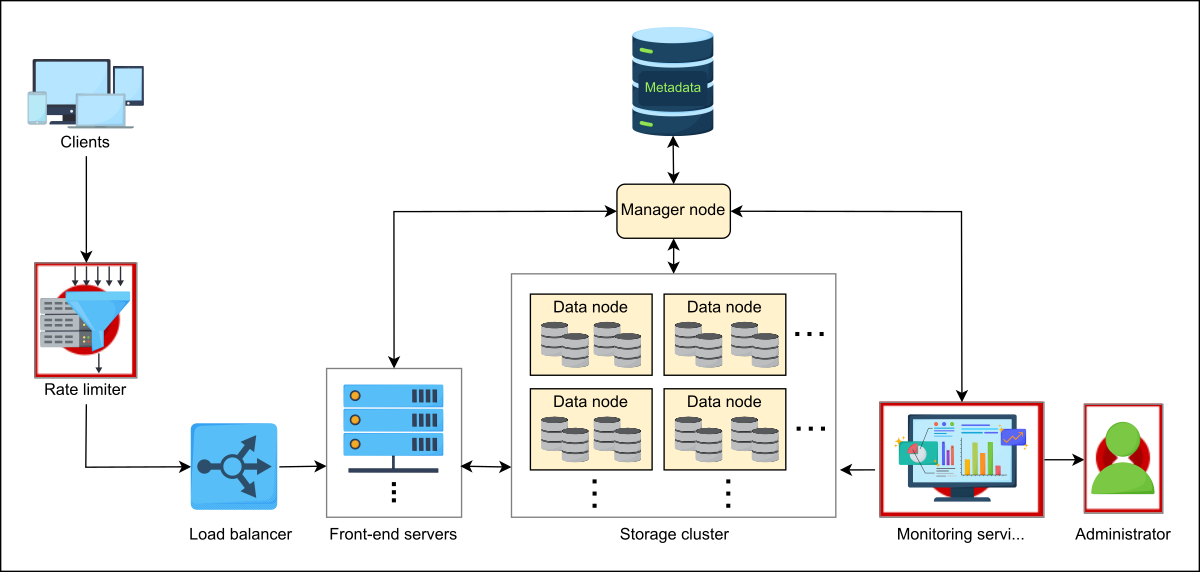
\includegraphics[width=0.5\textwidth]{Images/chapter_20/section_4910790825476096/6165646008516608.png}
 \caption{The detailed design of a blob store}
\end{figure}

\subsubsection{Workflow}\label{YENkyl3rmJbWMT75RyfYu}
\\
We describe the workflow based on the basic operations we can perform on a blob store. We assume that the user has successfully logged in and a container has already been created. A unique ID is assigned to each user and container. The user performs the following operations in a specific container.
\\
\textbf{Write a blob}

\begin{enumerate}
\item
\protect\phantomsection\label{cy-n9pIVoWXlp1AMNZ2GI}
The client generates the upload blob request. If the client's request successfully passes through the rate limiter, the load balancer forwards the client's request to one of the front-end servers. The front-end server then requests the manager node for the data nodes it should contact to store the blob.
\item
\protect\phantomsection\label{YAsFa8OQXjaFUu4RkEp05}
The manager node assigns the blob a unique ID using a \href{https://www.educative.io/courses/grokking-the-system-design-interview/design-of-a-unique-id-generator}{unique ID generator system}. It then splits the large-size blob into smaller, fixed-size chunks and assigns each chunk a data node where that chunk is eventually stored. The manager node determines the amount of storage space that's available on the data nodes using a \textbf{free-space management system}.
\item
\protect\phantomsection\label{CxDdB8yQ_p3TqxzSn_pHr}
After determining the mapping of chunks to data nodes, the front-end servers write the chunks to the assigned data nodes.
\item
\protect\phantomsection\label{kt7zIvGsmremPbw8dmdkG}
We replicate each chunk for redundancy purposes. All choices regarding chunk replication are made at the manager node. Hence , the manager node also allocates the storage and data nodes for storing replicas.
\item
\protect\phantomsection\label{E2tmP9GGoFeCViYAfV9oi}
The manager node stores the blob metadata in the metadata storage. We discuss the blob's metadata schema in detail in the next lesson.
\item
\protect\phantomsection\label{Mrzz50_pLOeuOJ72xfqQG}
After writing the blob, a fully qualified path of the blob is returned to the client. The path consists of the user ID, container ID where the user has added the blob, the blob ID, and the access level of the blob.
\end{enumerate}

\begin{quote}
\textbf{Quiz:}
\textbf{Question 1:} What does the manager node do if a user concurrently writes two blobs with the same name inside the same container?
\textbf{Answer:} The manager node serializes such operations and assigns a version number to the blob that's uploaded later.
\end{quote}

\textbf{Reading a blob}

\begin{enumerate}
\item
\protect\phantomsection\label{Gf-6ti_XA_hLb9kWyqtnM}
When a read request for a blob reaches the front-end server, it asks the manager node for that blob's metadata.
\item
\protect\phantomsection\label{PPQFrrLTDBQUSFhFOc9dV}
The manager node first checks whether that blob is private or public, based on the path of the blob and whether we're authorized to transfer that blob or not.
\item
\protect\phantomsection\label{wihk1vpP8PLLsMmRy7M3V}
After authorizing the blob, the manager node looks for the chunks for that blob in the metadata and looks at their mappings to data nodes. The manager node returns the chunks and their mappings (data nodes) to the client.
\item
\protect\phantomsection\label{ZV54X82RJFnSiwgI63Z7U}
The client then reads the chunk data from the data nodes.
\end{enumerate}
\begin{quote}
\textbf{Note:} The metadata information for reading the blob is cached at the client machine, so that the next time a client wants to read the same blob, we won't have to burden the manager node. Additionally, the client's read operation will be faster the next time.
\end{quote}

\begin{quote}
\textbf{Quiz:}
\textbf{Question 1:} Suppose the manager node moves data from one data node to another because of an impending disk failure. The user will now have stale information if they use the cached metadata to access the data. How do we handle such situations?
\textbf{Answer:} In such cases, the client calls fail. The client then flushes the cache and fetches new metadata information from the manager node.
\end{quote}

\textbf{Deleting a blob} Upon receiving a delete blob request, the manager node marks that blob as deleted in the metadata, and frees up the space later using a garbage collector. We learn more about garbage collectors in the next lesson.

\begin{quote}
\textbf{Quiz:}
\textbf{Question 1:} Can the manager node be considered a single point of failure? If yes,

then how can we cope with this problem?
\textbf{Answer:} Yes, because the manager node is the central point of a blob store and is a single point of failure. Therefore, we have to have a backup or shadow server in place of a manager node. The technique that we use for this is called checkpointing, meaning we take snapshots of the data at different time intervals. A snapshot captures the state, data, hardware configuration of the running manager node, and messages in transit between the manager and data nodes. It maintains the \#key\# operation log: A logical timeline, defining the serialized order of concurrent operations \#key\# in an external storage area or snapshot repository.

If the manager node fails, an automated system or the administrator uses the snapshot to restart that manager node from the state it failed at and replays the operation log.
\end{quote}

In the next lesson, we talk about the design considerations of a blob store.\\

% End of section content